\chapter{The History of X11: Triumphs and Legacy}
\label{ch:history-x11}

\epigraph{To understand where we're going, we must first understand where we've been.}{--- Wisdom of Software Evolution}

\section{Introduction}

Before we can fully appreciate Wayland, we need to understand its predecessor: the \textbf{X Window System}, commonly known as \textbf{X11} or simply \textbf{X}. For over three decades, X11 has been the foundation of graphical computing on Unix and Linux systems. Its story is one of remarkable longevity, clever design, and ultimately, the natural obsolescence that comes with changing technology.

This chapter is not a criticism of X11—quite the opposite. It's a celebration of an engineering marvel that served its purpose brilliantly for generations, and an honest examination of why even great systems eventually need replacement.

\section{The Birth of X: MIT in the 1980s}

\subsection{The Computing Landscape of 1984}

To understand X11, we need to travel back to 1984. The computing world was vastly different:

\begin{itemize}[leftmargin=*]
    \item Personal computers were just emerging (IBM PC was only 3 years old)
    \item Most computing happened on time-shared mainframes and minicomputers
    \item Terminals were often dumb—just keyboards and displays with no local processing
    \item Networks were slow by modern standards (measured in kilobits, not gigabits)
    \item Graphics acceleration didn't exist—CPUs did all the drawing
    \item Memory and storage were expensive and limited
\end{itemize}

\subsection{Project Athena}

In 1983, MIT launched Project Athena, an ambitious program to explore how computing could transform education. The project faced a fundamental problem: how could students and researchers access graphical applications from various terminals scattered across campus?

\begin{examplebox}
\textbf{The Problem Athena Needed to Solve}

Imagine a student sitting at a terminal in the library. They need to:
\begin{itemize}
    \item Run CAD software stored on an engineering department server
    \item Access email on a different machine
    \item Use a word processor on yet another system
    \item See everything on one screen
    \item Use one keyboard and mouse
\end{itemize}

All this over a relatively slow network, with the terminal itself having limited processing power.
\end{examplebox}

\subsection{The X Design Emerges}

Robert Scheifler and Jim Gettys at MIT created X to solve this problem. Their design made several crucial decisions:

\paragraph{1. Network Transparency from Day One}

Unlike earlier window systems designed for local use, X was built from the ground up to work over a network. This wasn't an afterthought—it was the primary design goal.

\paragraph{2. The X Philosophy}

The X design philosophy, as articulated in the early documentation, included several key principles:

\begin{principle}[Mechanism, Not Policy]
X provides mechanisms for building user interfaces but doesn't mandate how they should look or behave. Window manager behavior, look and feel, and user interface style are left to other components.
\end{principle}

\begin{principle}[No Assumptions About User Interface]
X doesn't impose any particular style of user interface. Whether you want overlapping windows or tiled layouts, fancy decorations or minimalism, X doesn't care.
\end{principle}

\begin{principle}[Network Transparency]
The protocol should work equally well whether the client and server are on the same machine or separated by a network.
\end{principle}

\begin{designbox}
\textbf{Why "Mechanism, Not Policy"?}

This principle reflects a deep wisdom about software architecture. By separating mechanism (what is possible) from policy (what should be done), X could:

\begin{itemize}
    \item Support multiple user interface styles
    \item Adapt to different workflows
    \item Evolve without protocol changes
    \item Let the best policies win through natural selection
\end{itemize}

This principle would later influence many other systems, including Wayland.
\end{designbox}

\subsection{The Client-Server Inversion}

One of X's most confusing aspects (which persists to this day) is the "backwards" nature of client and server:

\begin{itemize}[leftmargin=*]
    \item The \textbf{X server} runs on the machine with the display and keyboard
    \item The \textbf{X client} is the application, which might run on a different machine
\end{itemize}

This makes perfect sense in the original context: the server "serves" display services to clients (applications) that might be running remotely.

\begin{figure}[htbp]
\centering
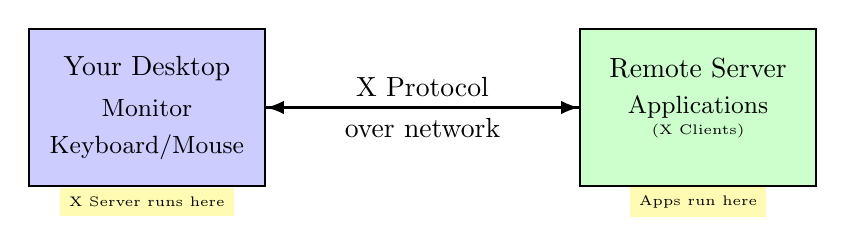
\begin{tikzpicture}[
    computer/.style={rectangle, draw, thick, minimum width=3cm, minimum height=2cm},
    arrow/.style={->, >=latex, very thick}
]
    % Local machine with display
    \node[computer, fill=blue!20] (local) at (0,0) {};
    \node at (0,0.5) {Your Desktop};
    \node[font=\small] at (0,0) {Monitor};
    \node[font=\small] at (0,-0.5) {Keyboard/Mouse};
    \node[font=\tiny, fill=yellow!30] at (0,-1.2) {X Server runs here};

    % Remote machine
    \node[computer, fill=green!20] (remote) at (7,0) {};
    \node at (7,0.5) {Remote Server};
    \node[font=\small] at (7,0) {Applications};
    \node[font=\tiny] at (7,-0.3) {(X Clients)};
    \node[font=\tiny, fill=yellow!30] at (7,-1.2) {Apps run here};

    % Network
    \draw[arrow] (remote.west) -- (local.east) node[midway, above] {X Protocol};
    \draw[arrow] (local.east) -- (remote.west) node[midway, below] {over network};
\end{tikzpicture}
\caption{X11's client-server model in the original networked context}
\label{fig:x11-network}
\end{figure}

\section{X11: The Protocol}

\subsection{Why "X11"?}

X went through several versions during development:
\begin{itemize}[leftmargin=*]
    \item X1 through X9 were development versions at MIT
    \item X10 was the first widely distributed version (1985)
    \item X11 was released in 1987 and became the standard
\end{itemize}

X11 has remained remarkably stable—the core protocol defined in 1987 is still in use today (with many extensions).

\subsection{The X11 Protocol Design}

The X11 protocol is based on asynchronous message passing:

\paragraph{Request and Reply}

Clients send \textbf{requests} to the server:
\begin{lstlisting}[style=cstyle]
// Example: Create a window
CreateWindow(
    window_id,      // Unique identifier
    parent_window,  // Parent window
    x, y,           // Position
    width, height,  // Size
    border_width,
    depth,
    class,
    visual,
    attributes
);
\end{lstlisting}

Some requests generate \textbf{replies}:
\begin{lstlisting}[style=cstyle]
// Example: Query pointer position
reply = QueryPointer(window_id);
// Reply contains: x, y, root_x, root_y, modifiers, etc.
\end{lstlisting}

\paragraph{Events}

The server sends \textbf{events} to clients asynchronously:
\begin{lstlisting}[style=cstyle]
// Events include:
// - KeyPress, KeyRelease
// - ButtonPress, ButtonRelease
// - MotionNotify (mouse movement)
// - EnterNotify, LeaveNotify (mouse entering/leaving window)
// - Expose (window needs repainting)
// - ConfigureNotify (window resized/moved)
// and many more...
\end{lstlisting}

\paragraph{Errors}

When something goes wrong, the server sends \textbf{error} messages.

\subsection{The X Server's Responsibilities}

In X11, the server has enormous responsibilities:

\begin{enumerate}[leftmargin=*]
    \item \textbf{Window Management Infrastructure}
    \begin{itemize}
        \item Maintaining the window hierarchy tree
        \item Tracking window positions and sizes
        \item Managing window properties
        \item Handling window stacking order
    \end{itemize}

    \item \textbf{Graphics Operations}
    \begin{itemize}
        \item Drawing primitives (lines, rectangles, arcs, etc.)
        \item Text rendering with fonts
        \item Image manipulation
        \item Graphics context management
    \end{itemize}

    \item \textbf{Input Handling}
    \begin{itemize}
        \item Capturing keyboard and mouse events
        \item Determining which window should receive events
        \item Managing keyboard focus
        \item Handling grabs (exclusive input capture)
    \end{itemize}

    \item \textbf{Resource Management}
    \begin{itemize}
        \item Managing server-side resources (pixmaps, fonts, cursors)
        \item Tracking client connections
        \item Coordinating access to hardware
    \end{itemize}

    \item \textbf{Display Management}
    \begin{itemize}
        \item Managing multiple screens
        \item Handling different visual types and color depths
        \item Managing the color map
    \end{itemize}
\end{enumerate}

\begin{importantbox}
The X server is a \textbf{monolithic} component. It does an enormous amount of work, which made sense in 1987 but would later become a source of problems.
\end{importantbox}

\section{X11's Clever Innovations}

X11 introduced many concepts that were revolutionary for their time and remain relevant:

\subsection{Network Transparency}

The ability to run applications remotely was genuinely transformative:

\begin{lstlisting}[language=bash]
# On your local machine
$ xhost +remotemachine

# SSH to remote machine
$ ssh remotemachine

# Run app remotely, display locally
$ export DISPLAY=yourmachine:0
$ firefox &
\end{lstlisting}

Firefox runs on the remote machine but displays on your local screen. In 1987, this was science fiction made real.

\subsection{Extensions}

X11 defined a mechanism for extending the protocol without breaking compatibility:

\begin{itemize}[leftmargin=*]
    \item Clients can query which extensions are available
    \item New features can be added without changing the core
    \item Older clients continue to work even if they don't know about new extensions
\end{itemize}

Major extensions include:
\begin{itemize}[leftmargin=*]
    \item \textbf{XSHM}: Shared memory for faster local performance
    \item \textbf{XRender}: Modern rendering model with anti-aliasing
    \item \textbf{GLX}: OpenGL integration
    \item \textbf{XRandR}: Runtime display reconfiguration
    \item \textbf{XInput}: Advanced input device support
    \item \textbf{Composite}: Window composition and effects
    \item \textbf{Xinerama/RandR}: Multi-monitor support
\end{itemize}

\subsection{Separation of Concerns}

X11's separation of the display server from the window manager was brilliant:

\begin{itemize}[leftmargin=*]
    \item Users could choose their preferred window manager
    \item Window manager development could proceed independently
    \item Different workflows could be accommodated
    \item Innovation could happen without changing the server
\end{itemize}

\subsection{The Root Window}

X11's concept of a root window (the background of the screen) that's just another window in the hierarchy was elegant:

\begin{itemize}[leftmargin=*]
    \item Consistent model throughout
    \item Easy to understand the window tree
    \item Simple to query and manipulate
\end{itemize}

\section{X11's Success and Dominance}

\subsection{The Rise of Linux}

While X11 started on commercial Unix systems, its real triumph came with Linux:

\begin{itemize}[leftmargin=*]
    \item \textbf{XFree86} (later \textbf{X.Org}) brought X11 to PC hardware
    \item Linux distributions standardized on X11
    \item GNOME and KDE built their desktops on X11
    \item X11 became synonymous with "graphical Linux"
\end{itemize}

\subsection{Portability}

X11 was ported to nearly every Unix-like system:
\begin{itemize}[leftmargin=*]
    \item Commercial Unix (Solaris, HP-UX, AIX, IRIX)
    \item BSD variants
    \item Linux
    \item Even macOS (via XQuartz)
\end{itemize}

\subsection{Application Ecosystem}

Decades of applications were built for X11:
\begin{itemize}[leftmargin=*]
    \item Scientific visualization tools
    \item CAD systems
    \item Office suites
    \item Web browsers
    \item Development environments
\end{itemize}

\section{The World Changes Around X11}

While X11 remained largely static (a testament to its design), the computing world transformed:

\subsection{Hardware Evolution}

\paragraph{1980s Hardware:}
\begin{itemize}[leftmargin=*]
    \item CPU does all rendering
    \item Simple framebuffers
    \item Limited memory
    \item Slow networks
    \item Single displays
\end{itemize}

\paragraph{2020s Hardware:}
\begin{itemize}[leftmargin=*]
    \item Powerful GPUs with hardware acceleration
    \item Complex memory hierarchies
    \item Abundant RAM
    \item Gigabit+ networks (or local-only use)
    \item Multiple high-resolution displays
    \item Touch screens
    \item Diverse input devices
\end{itemize}

\subsection{Usage Pattern Changes}

\paragraph{1980s Usage:}
\begin{itemize}[leftmargin=*]
    \item Network computing was essential
    \item Terminals accessing remote servers
    \item Text-heavy interfaces
    \item Limited graphics
\end{itemize}

\paragraph{2020s Usage:}
\begin{itemize}[leftmargin=*]
    \item Primarily local computing
    \item Network applications use custom protocols (VNC, RDP, web)
    \item Graphics-intensive interfaces
    \item Video, 3D, high-resolution images everywhere
    \item Composition effects expected
    \item Security and isolation critical
\end{itemize}

\subsection{Architectural Mismatches}

Several of X11's design decisions, brilliant in 1987, became problematic:

\paragraph{Network Transparency Overhead}

The protocol's network orientation adds overhead even for local use:
\begin{itemize}[leftmargin=*]
    \item Data must be serialized into protocol messages
    \item Extra copies of image data
    \item Synchronization complexity
    \item Can't take shortcuts available to local processes
\end{itemize}

\paragraph{Server-Side Rendering}

Having the server do rendering made sense with dumb terminals but became a bottleneck:
\begin{itemize}[leftmargin=*]
    \item Applications can't directly use GPU acceleration
    \item Every draw operation goes through the server
    \item Difficult to achieve optimal performance
    \item Hardware acceleration requires complex extensions (GLX)
\end{itemize}

\paragraph{Security Model}

X11's security model was designed for a trusted environment:
\begin{itemize}[leftmargin=*]
    \item Any client can read any window's pixels
    \item Clients can inject input to other clients
    \item Clients can read each other's properties
    \item Keylogging is trivial
\end{itemize}

This was acceptable when all users were trusted researchers at the same institution. It's unacceptable in the modern security landscape.

\begin{warningbox}
\textbf{The Keylogger Example}

In X11, any application can register to receive \textit{all} keyboard events, even those destined for other applications. A malicious program could easily record everything you type, including passwords.

While some protections have been added over the years, the fundamental architecture makes true security isolation impossible.
\end{warningbox}

\section{X11's Growing Pains}

\subsection{The Extension Explosion}

As X11 aged, more and more functionality was added via extensions:

\begin{itemize}[leftmargin=*]
    \item Over 30 major extensions
    \item Complexity grew enormously
    \item Interactions between extensions could be problematic
    \item Some extensions effectively created new sub-protocols
\end{itemize}

The clean, simple protocol of 1987 had become a sprawling complex system.

\subsection{The Composite Extension: A Turning Point}

The Composite extension, added in 2004, was particularly significant:

\begin{itemize}[leftmargin=*]
    \item Allowed window contents to be redirected to off-screen buffers
    \item Enabled a separate \textbf{compositing manager} to combine windows
    \item Made effects like transparency, shadows, and animations possible
\end{itemize}

\begin{figure}[htbp]
\centering
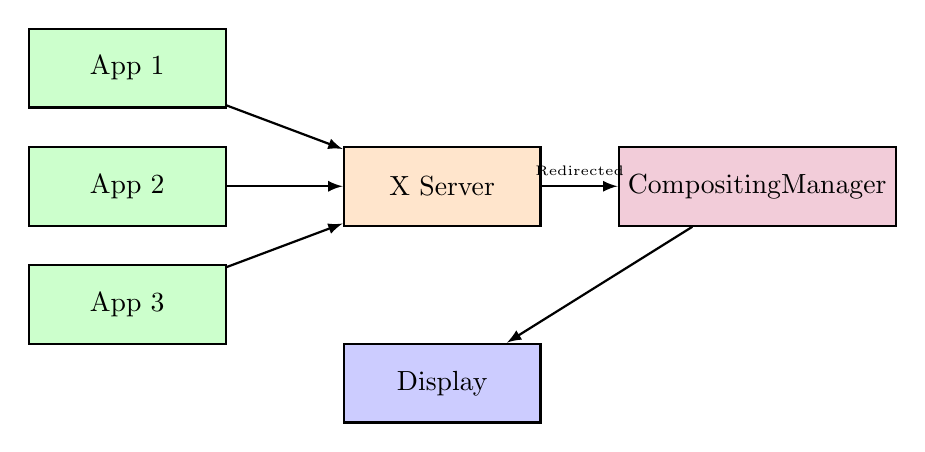
\begin{tikzpicture}[
    component/.style={rectangle, draw, thick, minimum width=2.5cm, minimum height=1cm},
    arrow/.style={->, >=latex, thick}
]
    \node[component, fill=green!20] (app1) at (0,4) {App 1};
    \node[component, fill=green!20] (app2) at (0,2.5) {App 2};
    \node[component, fill=green!20] (app3) at (0,1) {App 3};

    \node[component, fill=orange!20] (xserver) at (4,2.5) {X Server};

    \node[component, fill=purple!20] (compositor) at (8,2.5) {Compositing\\Manager};

    \node[component, fill=blue!20] (display) at (4,0) {Display};

    \draw[arrow] (app1) -- (xserver);
    \draw[arrow] (app2) -- (xserver);
    \draw[arrow] (app3) -- (xserver);
    \draw[arrow] (xserver) -- (compositor) node[midway, above, font=\tiny] {Redirected};
    \draw[arrow] (compositor) -- (display);
\end{tikzpicture}
\caption{X11 with compositing extension—the compositor is bolted on}
\label{fig:x11-composite}
\end{figure}

But compositing in X11 was \textit{bolted on}. The fundamental architecture still assumed direct rendering to the screen. This created complexity and inefficiency.

\subsection{The Code Complexity}

The X.Org server codebase grew to enormous size:
\begin{itemize}[leftmargin=*]
    \item Millions of lines of code
    \item Decades of accumulated complexity
    \item Difficult to modify without breaking something
    \item Steep learning curve for new developers
\end{itemize}

\section{Attempts at Reform}

Before Wayland, there were attempts to modernize X11:

\subsection{X11R6 and X11R7}

Various releases tried to improve X11:
\begin{itemize}[leftmargin=*]
    \item Modularization of the codebase
    \item Improved build system
    \item Better documentation
\end{itemize}

But the core architecture remained unchanged.

\subsection{The XCB Project}

XCB (X C Bindings) replaced Xlib with a cleaner, more efficient library:
\begin{itemize}[leftmargin=*]
    \item Better multi-threading support
    \item Reduced latency
    \item Cleaner API
\end{itemize}

But it was still X11 underneath.

\subsection{Why Reform Wasn't Enough}

The fundamental issue was that X11's core architecture, designed for 1987's computing environment, couldn't be incrementally updated to match modern needs:

\begin{itemize}[leftmargin=*]
    \item Network transparency built into every operation
    \item Server-side rendering model
    \item Lack of security isolation
    \item Composition as an afterthought
\end{itemize}

These weren't bugs—they were fundamental architectural decisions that had become liabilities.

\section{X11's Legacy}

\subsection{What X11 Got Right}

Despite its age, X11 taught us invaluable lessons:

\begin{enumerate}[leftmargin=*]
    \item \textbf{Mechanism, not policy}: Separate what's possible from what should be done
    \item \textbf{Extensibility}: Plan for future growth
    \item \textbf{Separation of concerns}: Display server, window manager, and applications should be separate
    \item \textbf{Flexibility}: Support diverse workflows and interfaces
    \item \textbf{Stability}: A good protocol can last decades
\end{enumerate}

\subsection{What X11 Teaches Us}

\begin{principle}[Design for Your Era]
X11 was perfectly designed for 1987. Its problems arose not from bad design, but from changed circumstances. Good design means solving today's problems, not yesterday's.
\end{principle}

\begin{principle}[Everything Has a Lifecycle]
Even excellent software eventually becomes obsolete. This is natural and healthy. The key is recognizing when it's time to move forward.
\end{principle}

\begin{principle}[Legacy Matters]
X11's longevity means it can't simply be turned off. Any successor must coexist with X11 for many years.
\end{principle}

\section{The Stage is Set for Wayland}

By the late 2000s, it was clear that:

\begin{itemize}[leftmargin=*]
    \item X11 had served admirably for over 20 years
    \item The computing landscape had fundamentally changed
    \item Incremental improvements weren't sufficient
    \item A new approach was needed
\end{itemize}

But what should that approach be?

The designers of Wayland learned from X11's successes and struggles:

\begin{itemize}[leftmargin=*]
    \item \textbf{Keep} the separation of mechanism and policy
    \item \textbf{Keep} the client-server model (but simplify it)
    \item \textbf{Drop} built-in network transparency
    \item \textbf{Make} composition first-class, not an extension
    \item \textbf{Design} for security from the start
    \item \textbf{Optimize} for the local case
    \item \textbf{Enable} direct hardware access for clients
    \item \textbf{Simplify} the core protocol
\end{itemize}

\section{Summary}

X11 is a triumph of software engineering:

\begin{itemize}[leftmargin=*]
    \item Designed in 1987, still in use in 2025
    \item Enabled the graphical Unix/Linux revolution
    \item Supported an incredible diversity of hardware and software
    \item Demonstrated the power of good abstractions
\end{itemize}

But it's also a cautionary tale:

\begin{itemize}[leftmargin=*]
    \item Optimization for one environment (networked computing) became a liability in another (local computing)
    \item Security models appropriate for trusted environments don't work in adversarial ones
    \item Even brilliant designs eventually need replacement
    \item Complexity accumulates over time
\end{itemize}

\begin{notebox}
\textbf{Key Takeaway}

X11 isn't bad—it's old. It solved 1987's problems brilliantly. But we now have 2025's problems, and they require 2025's solutions. That's where Wayland comes in.
\end{notebox}

In the next chapter, we'll examine X11's specific limitations in detail, setting the stage for understanding Wayland's different approach.

\section{Further Reading}

\begin{itemize}[leftmargin=*]
    \item "The X Window System" by Scheifler and Gettys (1986)
    \item X11 Protocol Specification
    \item "The X New Developer's Guide" by X.Org Foundation
    \item Historical papers from Project Athena
    \item Keith Packard's blog posts on X11 evolution
\end{itemize}
